\section{Homology test}\label{sec:homology}

\paragraph{Metric.} For a single chain, TCRs are grouped by epitope. Only
equal-length CDR3s can share a Hamming distance, so pairs are counted within
length bins. With $N_e$ TCRs for epitope $e$ in a cohort of $N$,
\[
P_{\text{self}}=\sum_e \binom{N_e}{2},\qquad
P_{\text{nonself}}=\binom{N}{2}-P_{\text{self}},
\]
(over equal-length pairs) and, writing $m_{\le d}$/$l_{\le d}$ for within-/between-epitope
pairs at Hamming $\le d$,
\[
\mathrm{S/N}(d)=\frac{m_{\le d}/P_{\text{self}}}{l_{\le d}/P_{\text{nonself}}}.
\]
The comparison is of \emph{rates}: non-self pairs vastly outnumber self pairs, so
raw counts are not comparable---only after normalising by $P_{\text{self}}$ and
$P_{\text{nonself}}$ does the enrichment appear. $d{=}0$ isolates publicity
(identical CDR3s); $d{=}1$ is the substitution-neighbour convergence signal
exploited by curated specificity databases~\cite{Shugay_2017}; signal $\Rightarrow$ S/N $\gg 1$, noise $\Rightarrow$
S/N $\approx 1$.

\paragraph{Result.} Figure~\ref{fig:hom} places the cohorts on the S/N axis at the
matched design. The ordering is
VDJdb-HQ $>$ TCRvdb-true $\gtrsim$ TCRvdb-false $>$ VDJdb-LQ $\gg$ immrep25 $>$ OLGA.
On TR$\beta$ the verified cohorts reach S/N $=\hqHomB$ (VDJdb-HQ) and $\trueHomB$
(TCRvdb-true), whereas immrep25 positives give only $\immHomB$ and the
$P_{\text{gen}}$-matched OLGA floor is $\olgaHomB$. The same picture holds on
TR$\alpha$ (immrep25 $\immHomA$ vs.\ OLGA $\olgaHomA$).

\begin{figure}[h]\centering
\begin{tikzpicture}[gnuplot]
%% generated with GNUPLOT 6.0p4 (Lua 5.5; terminal rev. Jun 2020, script rev. 120)
%% Sun Jul  5 18:01:10 2026
\tikzset{every node/.append style={font={\fontsize{8.0pt}{9.6pt}\selectfont}}}
\path (0.000,0.000) rectangle (16.000,8.000);
\gpcolor{color=gp lt color border}
\gpsetlinetype{gp lt border}
\gpsetdashtype{gp dt solid}
\gpsetlinewidth{1.00}
\draw[gp path] (1.348,1.033)--(1.438,1.033);
\draw[gp path] (7.558,1.033)--(7.468,1.033);
\draw[gp path] (1.348,1.136)--(1.438,1.136);
\draw[gp path] (7.558,1.136)--(7.468,1.136);
\draw[gp path] (1.348,1.223)--(1.438,1.223);
\draw[gp path] (7.558,1.223)--(7.468,1.223);
\draw[gp path] (1.348,1.299)--(1.438,1.299);
\draw[gp path] (7.558,1.299)--(7.468,1.299);
\draw[gp path] (1.348,1.366)--(1.438,1.366);
\draw[gp path] (7.558,1.366)--(7.468,1.366);
\gpcolor{rgb color={0.867,0.867,0.867}}
\gpsetlinetype{gp lt axes}
\gpsetdashtype{gp dt axes}
\gpsetlinewidth{0.50}
\draw[gp path] (1.348,1.425)--(7.558,1.425);
\gpcolor{color=gp lt color border}
\gpsetlinetype{gp lt border}
\gpsetdashtype{gp dt solid}
\gpsetlinewidth{1.00}
\draw[gp path] (1.348,1.425)--(1.528,1.425);
\draw[gp path] (7.558,1.425)--(7.378,1.425);
\node[gp node right] at (1.201,1.425) {$1$};
\draw[gp path] (1.348,1.818)--(1.438,1.818);
\draw[gp path] (7.558,1.818)--(7.468,1.818);
\draw[gp path] (1.348,2.047)--(1.438,2.047);
\draw[gp path] (7.558,2.047)--(7.468,2.047);
\draw[gp path] (1.348,2.210)--(1.438,2.210);
\draw[gp path] (7.558,2.210)--(7.468,2.210);
\draw[gp path] (1.348,2.336)--(1.438,2.336);
\draw[gp path] (7.558,2.336)--(7.468,2.336);
\draw[gp path] (1.348,2.440)--(1.438,2.440);
\draw[gp path] (7.558,2.440)--(7.468,2.440);
\draw[gp path] (1.348,2.527)--(1.438,2.527);
\draw[gp path] (7.558,2.527)--(7.468,2.527);
\draw[gp path] (1.348,2.602)--(1.438,2.602);
\draw[gp path] (7.558,2.602)--(7.468,2.602);
\draw[gp path] (1.348,2.669)--(1.438,2.669);
\draw[gp path] (7.558,2.669)--(7.468,2.669);
\gpcolor{rgb color={0.867,0.867,0.867}}
\gpsetlinetype{gp lt axes}
\gpsetdashtype{gp dt axes}
\gpsetlinewidth{0.50}
\draw[gp path] (1.348,2.729)--(7.558,2.729);
\gpcolor{color=gp lt color border}
\gpsetlinetype{gp lt border}
\gpsetdashtype{gp dt solid}
\gpsetlinewidth{1.00}
\draw[gp path] (1.348,2.729)--(1.528,2.729);
\draw[gp path] (7.558,2.729)--(7.378,2.729);
\node[gp node right] at (1.201,2.729) {$10$};
\draw[gp path] (1.348,3.121)--(1.438,3.121);
\draw[gp path] (7.558,3.121)--(7.468,3.121);
\draw[gp path] (1.348,3.351)--(1.438,3.351);
\draw[gp path] (7.558,3.351)--(7.468,3.351);
\draw[gp path] (1.348,3.514)--(1.438,3.514);
\draw[gp path] (7.558,3.514)--(7.468,3.514);
\draw[gp path] (1.348,3.640)--(1.438,3.640);
\draw[gp path] (7.558,3.640)--(7.468,3.640);
\draw[gp path] (1.348,3.743)--(1.438,3.743);
\draw[gp path] (7.558,3.743)--(7.468,3.743);
\draw[gp path] (1.348,3.830)--(1.438,3.830);
\draw[gp path] (7.558,3.830)--(7.468,3.830);
\draw[gp path] (1.348,3.906)--(1.438,3.906);
\draw[gp path] (7.558,3.906)--(7.468,3.906);
\draw[gp path] (1.348,3.973)--(1.438,3.973);
\draw[gp path] (7.558,3.973)--(7.468,3.973);
\gpcolor{rgb color={0.867,0.867,0.867}}
\gpsetlinetype{gp lt axes}
\gpsetdashtype{gp dt axes}
\gpsetlinewidth{0.50}
\draw[gp path] (1.348,4.032)--(7.558,4.032);
\gpcolor{color=gp lt color border}
\gpsetlinetype{gp lt border}
\gpsetdashtype{gp dt solid}
\gpsetlinewidth{1.00}
\draw[gp path] (1.348,4.032)--(1.528,4.032);
\draw[gp path] (7.558,4.032)--(7.378,4.032);
\node[gp node right] at (1.201,4.032) {$100$};
\draw[gp path] (1.348,4.425)--(1.438,4.425);
\draw[gp path] (7.558,4.425)--(7.468,4.425);
\draw[gp path] (1.348,4.654)--(1.438,4.654);
\draw[gp path] (7.558,4.654)--(7.468,4.654);
\draw[gp path] (1.348,4.817)--(1.438,4.817);
\draw[gp path] (7.558,4.817)--(7.468,4.817);
\draw[gp path] (1.348,4.943)--(1.438,4.943);
\draw[gp path] (7.558,4.943)--(7.468,4.943);
\draw[gp path] (1.348,5.047)--(1.438,5.047);
\draw[gp path] (7.558,5.047)--(7.468,5.047);
\draw[gp path] (1.348,5.134)--(1.438,5.134);
\draw[gp path] (7.558,5.134)--(7.468,5.134);
\draw[gp path] (1.348,5.209)--(1.438,5.209);
\draw[gp path] (7.558,5.209)--(7.468,5.209);
\draw[gp path] (1.348,5.276)--(1.438,5.276);
\draw[gp path] (7.558,5.276)--(7.468,5.276);
\gpcolor{rgb color={0.867,0.867,0.867}}
\gpsetlinetype{gp lt axes}
\gpsetdashtype{gp dt axes}
\gpsetlinewidth{0.50}
\draw[gp path] (1.348,5.336)--(7.558,5.336);
\gpcolor{color=gp lt color border}
\gpsetlinetype{gp lt border}
\gpsetdashtype{gp dt solid}
\gpsetlinewidth{1.00}
\draw[gp path] (1.348,5.336)--(1.528,5.336);
\draw[gp path] (7.558,5.336)--(7.378,5.336);
\node[gp node right] at (1.201,5.336) {$1000$};
\draw[gp path] (1.348,5.728)--(1.438,5.728);
\draw[gp path] (7.558,5.728)--(7.468,5.728);
\draw[gp path] (1.348,5.958)--(1.438,5.958);
\draw[gp path] (7.558,5.958)--(7.468,5.958);
\draw[gp path] (1.348,6.120)--(1.438,6.120);
\draw[gp path] (7.558,6.120)--(7.468,6.120);
\draw[gp path] (1.348,6.247)--(1.438,6.247);
\draw[gp path] (7.558,6.247)--(7.468,6.247);
\draw[gp path] (1.348,6.350)--(1.438,6.350);
\draw[gp path] (7.558,6.350)--(7.468,6.350);
\draw[gp path] (1.348,6.437)--(1.438,6.437);
\draw[gp path] (7.558,6.437)--(7.468,6.437);
\draw[gp path] (1.348,6.513)--(1.438,6.513);
\draw[gp path] (7.558,6.513)--(7.468,6.513);
\draw[gp path] (1.348,6.579)--(1.438,6.579);
\draw[gp path] (7.558,6.579)--(7.468,6.579);
\gpcolor{rgb color={0.867,0.867,0.867}}
\gpsetlinetype{gp lt axes}
\gpsetdashtype{gp dt axes}
\gpsetlinewidth{0.50}
\draw[gp path] (1.348,6.639)--(7.558,6.639);
\gpcolor{color=gp lt color border}
\gpsetlinetype{gp lt border}
\gpsetdashtype{gp dt solid}
\gpsetlinewidth{1.00}
\draw[gp path] (1.348,6.639)--(1.528,6.639);
\draw[gp path] (7.558,6.639)--(7.378,6.639);
\node[gp node right] at (1.201,6.639) {$10000$};
\draw[gp path] (1.348,7.031)--(1.438,7.031);
\draw[gp path] (7.558,7.031)--(7.468,7.031);
\draw[gp path] (1.348,7.261)--(1.438,7.261);
\draw[gp path] (7.558,7.261)--(7.468,7.261);
\draw[gp path] (1.753,1.033)--(1.753,0.853);
\node[gp node right,rotate=40.0,font={\fontsize{7.0pt}{8.4pt}\selectfont}] at (1.753,0.682) {TCRvdb true};
\draw[gp path] (2.428,1.033)--(2.428,0.853);
\node[gp node right,rotate=40.0,font={\fontsize{7.0pt}{8.4pt}\selectfont}] at (2.428,0.682) {VDJdb HQ};
\draw[gp path] (3.103,1.033)--(3.103,0.853);
\node[gp node right,rotate=40.0,font={\fontsize{7.0pt}{8.4pt}\selectfont}] at (3.103,0.682) {VDJdb LQ};
\draw[gp path] (3.778,1.033)--(3.778,0.853);
\node[gp node right,rotate=40.0,font={\fontsize{7.0pt}{8.4pt}\selectfont}] at (3.778,0.682) {TCRvdb false};
\draw[gp path] (4.453,1.033)--(4.453,0.853);
\node[gp node right,rotate=40.0,font={\fontsize{7.0pt}{8.4pt}\selectfont}] at (4.453,0.682) {immrep25};
\draw[gp path] (5.128,1.033)--(5.128,0.853);
\node[gp node right,rotate=40.0,font={\fontsize{7.0pt}{8.4pt}\selectfont}] at (5.128,0.682) {AIRR rand};
\draw[gp path] (5.803,1.033)--(5.803,0.853);
\node[gp node right,rotate=40.0,font={\fontsize{7.0pt}{8.4pt}\selectfont}] at (5.803,0.682) {AIRR nonrand};
\draw[gp path] (6.478,1.033)--(6.478,0.853);
\node[gp node right,rotate=40.0,font={\fontsize{7.0pt}{8.4pt}\selectfont}] at (6.478,0.682) {OLGA rand};
\draw[gp path] (7.153,1.033)--(7.153,0.853);
\node[gp node right,rotate=40.0,font={\fontsize{7.0pt}{8.4pt}\selectfont}] at (7.153,0.682) {MLR exp.\ $\beta$};
\draw[gp path] (1.348,7.261)--(1.348,1.033)--(7.558,1.033)--(7.558,7.261)--cycle;
\gpfill{rgb color={0.129,0.400,0.675},color=.!55} (1.517,1.033)--(1.990,1.033)--(1.990,5.355)--(1.517,5.355)--cycle;
\draw[gp path] (1.517,1.033)--(1.517,5.354)--(1.989,5.354)--(1.989,1.033)--cycle;
\gpfill{rgb color={0.129,0.400,0.675},color=.!55} (2.192,1.033)--(2.665,1.033)--(2.665,5.164)--(2.192,5.164)--cycle;
\draw[gp path] (2.192,1.033)--(2.192,5.163)--(2.664,5.163)--(2.664,1.033)--cycle;
\gpfill{rgb color={0.404,0.663,0.812},color=.!55} (2.867,1.033)--(3.340,1.033)--(3.340,3.156)--(2.867,3.156)--cycle;
\draw[gp path] (2.867,1.033)--(2.867,3.155)--(3.339,3.155)--(3.339,1.033)--cycle;
\gpfill{rgb color={0.698,0.094,0.169},color=.!55} (3.542,1.033)--(4.015,1.033)--(4.015,2.727)--(3.542,2.727)--cycle;
\draw[gp path] (3.542,1.033)--(3.542,2.726)--(4.014,2.726)--(4.014,1.033)--cycle;
\gpfill{rgb color={0.937,0.541,0.000},color=.!55} (4.217,1.033)--(4.690,1.033)--(4.690,2.194)--(4.217,2.194)--cycle;
\draw[gp path] (4.217,1.033)--(4.217,2.193)--(4.689,2.193)--(4.689,1.033)--cycle;
\gpfill{rgb color={0.620,0.604,0.784},color=.!55} (4.892,1.033)--(5.365,1.033)--(5.365,1.423)--(4.892,1.423)--cycle;
\draw[gp path] (4.892,1.033)--(4.892,1.422)--(5.364,1.422)--(5.364,1.033)--cycle;
\gpfill{rgb color={0.416,0.318,0.639},color=.!55} (5.567,1.033)--(6.040,1.033)--(6.040,1.458)--(5.567,1.458)--cycle;
\draw[gp path] (5.567,1.033)--(5.567,1.457)--(6.039,1.457)--(6.039,1.033)--cycle;
\gpfill{rgb color={0.698,0.094,0.169},color=.!55} (6.242,1.033)--(6.715,1.033)--(6.715,1.422)--(6.242,1.422)--cycle;
\draw[gp path] (6.242,1.033)--(6.242,1.421)--(6.714,1.421)--(6.714,1.033)--cycle;
\gpcolor{rgb color={0.000,0.000,0.000}}
\draw[gp path] (1.753,5.328)--(1.753,5.381);
\draw[gp path] (1.663,5.328)--(1.843,5.328);
\draw[gp path] (1.663,5.381)--(1.843,5.381);
\draw[gp path] (2.428,3.726)--(2.428,6.599);
\draw[gp path] (2.338,3.726)--(2.518,3.726);
\draw[gp path] (2.338,6.599)--(2.518,6.599);
\draw[gp path] (3.103,2.921)--(3.103,3.389);
\draw[gp path] (3.013,2.921)--(3.193,2.921);
\draw[gp path] (3.013,3.389)--(3.193,3.389);
\draw[gp path] (3.778,1.071)--(3.778,4.380);
\draw[gp path] (3.688,1.071)--(3.868,1.071);
\draw[gp path] (3.688,4.380)--(3.868,4.380);
\draw[gp path] (4.453,2.009)--(4.453,2.378);
\draw[gp path] (4.363,2.009)--(4.543,2.009);
\draw[gp path] (4.363,2.378)--(4.543,2.378);
\draw[gp path] (5.128,1.419)--(5.128,1.426);
\draw[gp path] (5.038,1.419)--(5.218,1.419);
\draw[gp path] (5.038,1.426)--(5.218,1.426);
\draw[gp path] (5.803,1.298)--(5.803,1.615);
\draw[gp path] (5.713,1.298)--(5.893,1.298);
\draw[gp path] (5.713,1.615)--(5.893,1.615);
\draw[gp path] (6.478,1.330)--(6.478,1.511);
\draw[gp path] (6.388,1.330)--(6.568,1.330);
\draw[gp path] (6.388,1.511)--(6.568,1.511);
\gpcolor{color=gpbgfillcolor}
\gpsetpointsize{4.00}
\gp3point{gp mark 7}{}{(1.753,5.354)}
\gpcolor{rgb color={0.000,0.000,0.000}}
\gpsetpointsize{2.00}
\gp3point{gp mark 7}{}{(1.753,5.354)}
\gpcolor{color=gpbgfillcolor}
\gpsetpointsize{4.00}
\gp3point{gp mark 7}{}{(2.428,5.163)}
\gpcolor{rgb color={0.000,0.000,0.000}}
\gpsetpointsize{2.00}
\gp3point{gp mark 7}{}{(2.428,5.163)}
\gpcolor{color=gpbgfillcolor}
\gpsetpointsize{4.00}
\gp3point{gp mark 7}{}{(3.103,3.155)}
\gpcolor{rgb color={0.000,0.000,0.000}}
\gpsetpointsize{2.00}
\gp3point{gp mark 7}{}{(3.103,3.155)}
\gpcolor{color=gpbgfillcolor}
\gpsetpointsize{4.00}
\gp3point{gp mark 7}{}{(3.778,2.726)}
\gpcolor{rgb color={0.000,0.000,0.000}}
\gpsetpointsize{2.00}
\gp3point{gp mark 7}{}{(3.778,2.726)}
\gpcolor{color=gpbgfillcolor}
\gpsetpointsize{4.00}
\gp3point{gp mark 7}{}{(4.453,2.193)}
\gpcolor{rgb color={0.000,0.000,0.000}}
\gpsetpointsize{2.00}
\gp3point{gp mark 7}{}{(4.453,2.193)}
\gpcolor{color=gpbgfillcolor}
\gpsetpointsize{4.00}
\gp3point{gp mark 7}{}{(5.128,1.422)}
\gpcolor{rgb color={0.000,0.000,0.000}}
\gpsetpointsize{2.00}
\gp3point{gp mark 7}{}{(5.128,1.422)}
\gpcolor{color=gpbgfillcolor}
\gpsetpointsize{4.00}
\gp3point{gp mark 7}{}{(5.803,1.457)}
\gpcolor{rgb color={0.000,0.000,0.000}}
\gpsetpointsize{2.00}
\gp3point{gp mark 7}{}{(5.803,1.457)}
\gpcolor{color=gpbgfillcolor}
\gpsetpointsize{4.00}
\gp3point{gp mark 7}{}{(6.478,1.421)}
\gpcolor{rgb color={0.000,0.000,0.000}}
\gpsetpointsize{2.00}
\gp3point{gp mark 7}{}{(6.478,1.421)}
\gpcolor{rgb color={0.267,0.267,0.267}}
\gpsetdashtype{gp dt 2}
\draw[gp path] (1.348,1.425)--(1.411,1.425)--(1.473,1.425)--(1.536,1.425)--(1.599,1.425)%
  --(1.662,1.425)--(1.724,1.425)--(1.787,1.425)--(1.850,1.425)--(1.913,1.425)--(1.975,1.425)%
  --(2.038,1.425)--(2.101,1.425)--(2.163,1.425)--(2.226,1.425)--(2.289,1.425)--(2.352,1.425)%
  --(2.414,1.425)--(2.477,1.425)--(2.540,1.425)--(2.603,1.425)--(2.665,1.425)--(2.728,1.425)%
  --(2.791,1.425)--(2.853,1.425)--(2.916,1.425)--(2.979,1.425)--(3.042,1.425)--(3.104,1.425)%
  --(3.167,1.425)--(3.230,1.425)--(3.293,1.425)--(3.355,1.425)--(3.418,1.425)--(3.481,1.425)%
  --(3.543,1.425)--(3.606,1.425)--(3.669,1.425)--(3.732,1.425)--(3.794,1.425)--(3.857,1.425)%
  --(3.920,1.425)--(3.983,1.425)--(4.045,1.425)--(4.108,1.425)--(4.171,1.425)--(4.233,1.425)%
  --(4.296,1.425)--(4.359,1.425)--(4.422,1.425)--(4.484,1.425)--(4.547,1.425)--(4.610,1.425)%
  --(4.673,1.425)--(4.735,1.425)--(4.798,1.425)--(4.861,1.425)--(4.923,1.425)--(4.986,1.425)%
  --(5.049,1.425)--(5.112,1.425)--(5.174,1.425)--(5.237,1.425)--(5.300,1.425)--(5.363,1.425)%
  --(5.425,1.425)--(5.488,1.425)--(5.551,1.425)--(5.613,1.425)--(5.676,1.425)--(5.739,1.425)%
  --(5.802,1.425)--(5.864,1.425)--(5.927,1.425)--(5.990,1.425)--(6.053,1.425)--(6.115,1.425)%
  --(6.178,1.425)--(6.241,1.425)--(6.303,1.425)--(6.366,1.425)--(6.429,1.425)--(6.492,1.425)%
  --(6.554,1.425)--(6.617,1.425)--(6.680,1.425)--(6.743,1.425)--(6.805,1.425)--(6.868,1.425)%
  --(6.931,1.425)--(6.993,1.425)--(7.056,1.425)--(7.119,1.425)--(7.182,1.425)--(7.244,1.425)%
  --(7.307,1.425)--(7.370,1.425)--(7.433,1.425)--(7.495,1.425)--(7.558,1.425);
\gpcolor{color=gp lt color border}
\gpsetdashtype{gp dt solid}
\draw[gp path] (1.348,7.261)--(1.348,1.033)--(7.558,1.033)--(7.558,7.261)--cycle;
\node[gp node center,rotate=-270.0,font={\fontsize{8.0pt}{9.6pt}\selectfont}] at (0.232,4.147) {homology S/N (self / non-self, $d{=}1$)};
\node[gp node center,font={\fontsize{8.0pt}{9.6pt}\selectfont}] at (4.453,7.630) {TCR$\alpha$};
%% coordinates of the plot area
\gpdefrectangularnode{gp plot 1}{\pgfpoint{1.348cm}{1.033cm}}{\pgfpoint{7.558cm}{7.261cm}}
\draw[gp path] (9.348,1.033)--(9.438,1.033);
\draw[gp path] (15.030,1.033)--(14.940,1.033);
\draw[gp path] (9.348,1.136)--(9.438,1.136);
\draw[gp path] (15.030,1.136)--(14.940,1.136);
\draw[gp path] (9.348,1.223)--(9.438,1.223);
\draw[gp path] (15.030,1.223)--(14.940,1.223);
\draw[gp path] (9.348,1.299)--(9.438,1.299);
\draw[gp path] (15.030,1.299)--(14.940,1.299);
\draw[gp path] (9.348,1.366)--(9.438,1.366);
\draw[gp path] (15.030,1.366)--(14.940,1.366);
\gpcolor{rgb color={0.867,0.867,0.867}}
\gpsetlinetype{gp lt axes}
\gpsetdashtype{gp dt axes}
\gpsetlinewidth{0.50}
\draw[gp path] (9.348,1.425)--(15.030,1.425);
\gpcolor{color=gp lt color border}
\gpsetlinetype{gp lt border}
\gpsetdashtype{gp dt solid}
\gpsetlinewidth{1.00}
\draw[gp path] (9.348,1.425)--(9.528,1.425);
\draw[gp path] (15.030,1.425)--(14.850,1.425);
\node[gp node right,font={\fontsize{8.0pt}{9.6pt}\selectfont}] at (9.201,1.425) {$1$};
\draw[gp path] (9.348,1.818)--(9.438,1.818);
\draw[gp path] (15.030,1.818)--(14.940,1.818);
\draw[gp path] (9.348,2.047)--(9.438,2.047);
\draw[gp path] (15.030,2.047)--(14.940,2.047);
\draw[gp path] (9.348,2.210)--(9.438,2.210);
\draw[gp path] (15.030,2.210)--(14.940,2.210);
\draw[gp path] (9.348,2.336)--(9.438,2.336);
\draw[gp path] (15.030,2.336)--(14.940,2.336);
\draw[gp path] (9.348,2.440)--(9.438,2.440);
\draw[gp path] (15.030,2.440)--(14.940,2.440);
\draw[gp path] (9.348,2.527)--(9.438,2.527);
\draw[gp path] (15.030,2.527)--(14.940,2.527);
\draw[gp path] (9.348,2.602)--(9.438,2.602);
\draw[gp path] (15.030,2.602)--(14.940,2.602);
\draw[gp path] (9.348,2.669)--(9.438,2.669);
\draw[gp path] (15.030,2.669)--(14.940,2.669);
\gpcolor{rgb color={0.867,0.867,0.867}}
\gpsetlinetype{gp lt axes}
\gpsetdashtype{gp dt axes}
\gpsetlinewidth{0.50}
\draw[gp path] (9.348,2.729)--(15.030,2.729);
\gpcolor{color=gp lt color border}
\gpsetlinetype{gp lt border}
\gpsetdashtype{gp dt solid}
\gpsetlinewidth{1.00}
\draw[gp path] (9.348,2.729)--(9.528,2.729);
\draw[gp path] (15.030,2.729)--(14.850,2.729);
\node[gp node right,font={\fontsize{8.0pt}{9.6pt}\selectfont}] at (9.201,2.729) {$10$};
\draw[gp path] (9.348,3.121)--(9.438,3.121);
\draw[gp path] (15.030,3.121)--(14.940,3.121);
\draw[gp path] (9.348,3.351)--(9.438,3.351);
\draw[gp path] (15.030,3.351)--(14.940,3.351);
\draw[gp path] (9.348,3.514)--(9.438,3.514);
\draw[gp path] (15.030,3.514)--(14.940,3.514);
\draw[gp path] (9.348,3.640)--(9.438,3.640);
\draw[gp path] (15.030,3.640)--(14.940,3.640);
\draw[gp path] (9.348,3.743)--(9.438,3.743);
\draw[gp path] (15.030,3.743)--(14.940,3.743);
\draw[gp path] (9.348,3.830)--(9.438,3.830);
\draw[gp path] (15.030,3.830)--(14.940,3.830);
\draw[gp path] (9.348,3.906)--(9.438,3.906);
\draw[gp path] (15.030,3.906)--(14.940,3.906);
\draw[gp path] (9.348,3.973)--(9.438,3.973);
\draw[gp path] (15.030,3.973)--(14.940,3.973);
\gpcolor{rgb color={0.867,0.867,0.867}}
\gpsetlinetype{gp lt axes}
\gpsetdashtype{gp dt axes}
\gpsetlinewidth{0.50}
\draw[gp path] (9.348,4.032)--(15.030,4.032);
\gpcolor{color=gp lt color border}
\gpsetlinetype{gp lt border}
\gpsetdashtype{gp dt solid}
\gpsetlinewidth{1.00}
\draw[gp path] (9.348,4.032)--(9.528,4.032);
\draw[gp path] (15.030,4.032)--(14.850,4.032);
\node[gp node right,font={\fontsize{8.0pt}{9.6pt}\selectfont}] at (9.201,4.032) {$100$};
\draw[gp path] (9.348,4.425)--(9.438,4.425);
\draw[gp path] (15.030,4.425)--(14.940,4.425);
\draw[gp path] (9.348,4.654)--(9.438,4.654);
\draw[gp path] (15.030,4.654)--(14.940,4.654);
\draw[gp path] (9.348,4.817)--(9.438,4.817);
\draw[gp path] (15.030,4.817)--(14.940,4.817);
\draw[gp path] (9.348,4.943)--(9.438,4.943);
\draw[gp path] (15.030,4.943)--(14.940,4.943);
\draw[gp path] (9.348,5.047)--(9.438,5.047);
\draw[gp path] (15.030,5.047)--(14.940,5.047);
\draw[gp path] (9.348,5.134)--(9.438,5.134);
\draw[gp path] (15.030,5.134)--(14.940,5.134);
\draw[gp path] (9.348,5.209)--(9.438,5.209);
\draw[gp path] (15.030,5.209)--(14.940,5.209);
\draw[gp path] (9.348,5.276)--(9.438,5.276);
\draw[gp path] (15.030,5.276)--(14.940,5.276);
\gpcolor{rgb color={0.867,0.867,0.867}}
\gpsetlinetype{gp lt axes}
\gpsetdashtype{gp dt axes}
\gpsetlinewidth{0.50}
\draw[gp path] (9.348,5.336)--(15.030,5.336);
\gpcolor{color=gp lt color border}
\gpsetlinetype{gp lt border}
\gpsetdashtype{gp dt solid}
\gpsetlinewidth{1.00}
\draw[gp path] (9.348,5.336)--(9.528,5.336);
\draw[gp path] (15.030,5.336)--(14.850,5.336);
\node[gp node right,font={\fontsize{8.0pt}{9.6pt}\selectfont}] at (9.201,5.336) {$1000$};
\draw[gp path] (9.348,5.728)--(9.438,5.728);
\draw[gp path] (15.030,5.728)--(14.940,5.728);
\draw[gp path] (9.348,5.958)--(9.438,5.958);
\draw[gp path] (15.030,5.958)--(14.940,5.958);
\draw[gp path] (9.348,6.120)--(9.438,6.120);
\draw[gp path] (15.030,6.120)--(14.940,6.120);
\draw[gp path] (9.348,6.247)--(9.438,6.247);
\draw[gp path] (15.030,6.247)--(14.940,6.247);
\draw[gp path] (9.348,6.350)--(9.438,6.350);
\draw[gp path] (15.030,6.350)--(14.940,6.350);
\draw[gp path] (9.348,6.437)--(9.438,6.437);
\draw[gp path] (15.030,6.437)--(14.940,6.437);
\draw[gp path] (9.348,6.513)--(9.438,6.513);
\draw[gp path] (15.030,6.513)--(14.940,6.513);
\draw[gp path] (9.348,6.579)--(9.438,6.579);
\draw[gp path] (15.030,6.579)--(14.940,6.579);
\gpcolor{rgb color={0.867,0.867,0.867}}
\gpsetlinetype{gp lt axes}
\gpsetdashtype{gp dt axes}
\gpsetlinewidth{0.50}
\draw[gp path] (9.348,6.639)--(15.030,6.639);
\gpcolor{color=gp lt color border}
\gpsetlinetype{gp lt border}
\gpsetdashtype{gp dt solid}
\gpsetlinewidth{1.00}
\draw[gp path] (9.348,6.639)--(9.528,6.639);
\draw[gp path] (15.030,6.639)--(14.850,6.639);
\node[gp node right,font={\fontsize{8.0pt}{9.6pt}\selectfont}] at (9.201,6.639) {$10000$};
\draw[gp path] (9.348,7.031)--(9.438,7.031);
\draw[gp path] (15.030,7.031)--(14.940,7.031);
\draw[gp path] (9.348,7.261)--(9.438,7.261);
\draw[gp path] (15.030,7.261)--(14.940,7.261);
\draw[gp path] (9.719,1.033)--(9.719,0.853);
\node[gp node right,rotate=40.0,font={\fontsize{7.0pt}{8.4pt}\selectfont}] at (9.719,0.682) {TCRvdb true};
\draw[gp path] (10.336,1.033)--(10.336,0.853);
\node[gp node right,rotate=40.0,font={\fontsize{7.0pt}{8.4pt}\selectfont}] at (10.336,0.682) {VDJdb HQ};
\draw[gp path] (10.954,1.033)--(10.954,0.853);
\node[gp node right,rotate=40.0,font={\fontsize{7.0pt}{8.4pt}\selectfont}] at (10.954,0.682) {VDJdb LQ};
\draw[gp path] (11.571,1.033)--(11.571,0.853);
\node[gp node right,rotate=40.0,font={\fontsize{7.0pt}{8.4pt}\selectfont}] at (11.571,0.682) {TCRvdb false};
\draw[gp path] (12.189,1.033)--(12.189,0.853);
\node[gp node right,rotate=40.0,font={\fontsize{7.0pt}{8.4pt}\selectfont}] at (12.189,0.682) {immrep25};
\draw[gp path] (12.807,1.033)--(12.807,0.853);
\node[gp node right,rotate=40.0,font={\fontsize{7.0pt}{8.4pt}\selectfont}] at (12.807,0.682) {AIRR rand};
\draw[gp path] (13.424,1.033)--(13.424,0.853);
\node[gp node right,rotate=40.0,font={\fontsize{7.0pt}{8.4pt}\selectfont}] at (13.424,0.682) {AIRR nonrand};
\draw[gp path] (14.042,1.033)--(14.042,0.853);
\node[gp node right,rotate=40.0,font={\fontsize{7.0pt}{8.4pt}\selectfont}] at (14.042,0.682) {OLGA rand};
\draw[gp path] (14.659,1.033)--(14.659,0.853);
\node[gp node right,rotate=40.0,font={\fontsize{7.0pt}{8.4pt}\selectfont}] at (14.659,0.682) {MLR exp.\ $\beta$};
\draw[gp path] (9.348,7.261)--(9.348,1.033)--(15.030,1.033)--(15.030,7.261)--cycle;
\gpfill{rgb color={0.129,0.400,0.675},color=.!55} (9.502,1.033)--(9.936,1.033)--(9.936,4.939)--(9.502,4.939)--cycle;
\draw[gp path] (9.502,1.033)--(9.502,4.938)--(9.935,4.938)--(9.935,1.033)--cycle;
\gpfill{rgb color={0.129,0.400,0.675},color=.!55} (10.120,1.033)--(10.553,1.033)--(10.553,5.655)--(10.120,5.655)--cycle;
\draw[gp path] (10.120,1.033)--(10.120,5.654)--(10.552,5.654)--(10.552,1.033)--cycle;
\gpfill{rgb color={0.404,0.663,0.812},color=.!55} (10.738,1.033)--(11.171,1.033)--(11.171,3.346)--(10.738,3.346)--cycle;
\draw[gp path] (10.738,1.033)--(10.738,3.345)--(11.170,3.345)--(11.170,1.033)--cycle;
\gpfill{rgb color={0.698,0.094,0.169},color=.!55} (11.355,1.033)--(11.789,1.033)--(11.789,3.947)--(11.355,3.947)--cycle;
\draw[gp path] (11.355,1.033)--(11.355,3.946)--(11.788,3.946)--(11.788,1.033)--cycle;
\gpfill{rgb color={0.937,0.541,0.000},color=.!55} (11.973,1.033)--(12.406,1.033)--(12.406,1.988)--(11.973,1.988)--cycle;
\draw[gp path] (11.973,1.033)--(11.973,1.987)--(12.405,1.987)--(12.405,1.033)--cycle;
\gpfill{rgb color={0.620,0.604,0.784},color=.!55} (12.590,1.033)--(13.024,1.033)--(13.024,1.426)--(12.590,1.426)--cycle;
\draw[gp path] (12.590,1.033)--(12.590,1.425)--(13.023,1.425)--(13.023,1.033)--cycle;
\gpfill{rgb color={0.416,0.318,0.639},color=.!55} (13.208,1.033)--(13.641,1.033)--(13.641,1.450)--(13.208,1.450)--cycle;
\draw[gp path] (13.208,1.033)--(13.208,1.449)--(13.640,1.449)--(13.640,1.033)--cycle;
\gpfill{rgb color={0.698,0.094,0.169},color=.!55} (13.826,1.033)--(14.259,1.033)--(14.259,1.409)--(13.826,1.409)--cycle;
\draw[gp path] (13.826,1.033)--(13.826,1.408)--(14.258,1.408)--(14.258,1.033)--cycle;
\gpfill{rgb color={0.208,0.592,0.561},color=.!55} (14.443,1.033)--(14.877,1.033)--(14.877,1.785)--(14.443,1.785)--cycle;
\draw[gp path] (14.443,1.033)--(14.443,1.784)--(14.876,1.784)--(14.876,1.033)--cycle;
\gpcolor{rgb color={0.000,0.000,0.000}}
\draw[gp path] (9.719,4.858)--(9.719,5.019);
\draw[gp path] (9.629,4.858)--(9.809,4.858);
\draw[gp path] (9.629,5.019)--(9.809,5.019);
\draw[gp path] (10.336,4.383)--(10.336,6.926);
\draw[gp path] (10.246,4.383)--(10.426,4.383);
\draw[gp path] (10.246,6.926)--(10.426,6.926);
\draw[gp path] (10.954,3.170)--(10.954,3.519);
\draw[gp path] (10.864,3.170)--(11.044,3.170);
\draw[gp path] (10.864,3.519)--(11.044,3.519);
\draw[gp path] (11.571,3.566)--(11.571,4.326);
\draw[gp path] (11.481,3.566)--(11.661,3.566);
\draw[gp path] (11.481,4.326)--(11.661,4.326);
\draw[gp path] (12.189,1.697)--(12.189,2.276);
\draw[gp path] (12.099,1.697)--(12.279,1.697);
\draw[gp path] (12.099,2.276)--(12.279,2.276);
\draw[gp path] (12.717,1.425)--(12.897,1.425);
\draw[gp path] (12.717,1.425)--(12.897,1.425);
\draw[gp path] (13.424,1.362)--(13.424,1.535);
\draw[gp path] (13.334,1.362)--(13.514,1.362);
\draw[gp path] (13.334,1.535)--(13.514,1.535);
\draw[gp path] (14.042,1.399)--(14.042,1.417);
\draw[gp path] (13.952,1.399)--(14.132,1.399);
\draw[gp path] (13.952,1.417)--(14.132,1.417);
\draw[gp path] (14.659,1.556)--(14.659,2.011);
\draw[gp path] (14.569,1.556)--(14.749,1.556);
\draw[gp path] (14.569,2.011)--(14.749,2.011);
\gpcolor{color=gpbgfillcolor}
\gpsetpointsize{4.00}
\gp3point{gp mark 7}{}{(9.719,4.938)}
\gpcolor{rgb color={0.000,0.000,0.000}}
\gpsetpointsize{2.00}
\gp3point{gp mark 7}{}{(9.719,4.938)}
\gpcolor{color=gpbgfillcolor}
\gpsetpointsize{4.00}
\gp3point{gp mark 7}{}{(10.336,5.654)}
\gpcolor{rgb color={0.000,0.000,0.000}}
\gpsetpointsize{2.00}
\gp3point{gp mark 7}{}{(10.336,5.654)}
\gpcolor{color=gpbgfillcolor}
\gpsetpointsize{4.00}
\gp3point{gp mark 7}{}{(10.954,3.345)}
\gpcolor{rgb color={0.000,0.000,0.000}}
\gpsetpointsize{2.00}
\gp3point{gp mark 7}{}{(10.954,3.345)}
\gpcolor{color=gpbgfillcolor}
\gpsetpointsize{4.00}
\gp3point{gp mark 7}{}{(11.571,3.946)}
\gpcolor{rgb color={0.000,0.000,0.000}}
\gpsetpointsize{2.00}
\gp3point{gp mark 7}{}{(11.571,3.946)}
\gpcolor{color=gpbgfillcolor}
\gpsetpointsize{4.00}
\gp3point{gp mark 7}{}{(12.189,1.987)}
\gpcolor{rgb color={0.000,0.000,0.000}}
\gpsetpointsize{2.00}
\gp3point{gp mark 7}{}{(12.189,1.987)}
\gpcolor{color=gpbgfillcolor}
\gpsetpointsize{4.00}
\gp3point{gp mark 7}{}{(12.807,1.425)}
\gpcolor{rgb color={0.000,0.000,0.000}}
\gpsetpointsize{2.00}
\gp3point{gp mark 7}{}{(12.807,1.425)}
\gpcolor{color=gpbgfillcolor}
\gpsetpointsize{4.00}
\gp3point{gp mark 7}{}{(13.424,1.449)}
\gpcolor{rgb color={0.000,0.000,0.000}}
\gpsetpointsize{2.00}
\gp3point{gp mark 7}{}{(13.424,1.449)}
\gpcolor{color=gpbgfillcolor}
\gpsetpointsize{4.00}
\gp3point{gp mark 7}{}{(14.042,1.408)}
\gpcolor{rgb color={0.000,0.000,0.000}}
\gpsetpointsize{2.00}
\gp3point{gp mark 7}{}{(14.042,1.408)}
\gpcolor{color=gpbgfillcolor}
\gpsetpointsize{4.00}
\gp3point{gp mark 7}{}{(14.659,1.784)}
\gpcolor{rgb color={0.000,0.000,0.000}}
\gpsetpointsize{2.00}
\gp3point{gp mark 7}{}{(14.659,1.784)}
\gpcolor{rgb color={0.267,0.267,0.267}}
\gpsetdashtype{gp dt 2}
\draw[gp path] (9.348,1.425)--(9.405,1.425)--(9.463,1.425)--(9.520,1.425)--(9.578,1.425)%
  --(9.635,1.425)--(9.692,1.425)--(9.750,1.425)--(9.807,1.425)--(9.865,1.425)--(9.922,1.425)%
  --(9.979,1.425)--(10.037,1.425)--(10.094,1.425)--(10.152,1.425)--(10.209,1.425)--(10.266,1.425)%
  --(10.324,1.425)--(10.381,1.425)--(10.438,1.425)--(10.496,1.425)--(10.553,1.425)--(10.611,1.425)%
  --(10.668,1.425)--(10.725,1.425)--(10.783,1.425)--(10.840,1.425)--(10.898,1.425)--(10.955,1.425)%
  --(11.012,1.425)--(11.070,1.425)--(11.127,1.425)--(11.185,1.425)--(11.242,1.425)--(11.299,1.425)%
  --(11.357,1.425)--(11.414,1.425)--(11.472,1.425)--(11.529,1.425)--(11.586,1.425)--(11.644,1.425)%
  --(11.701,1.425)--(11.759,1.425)--(11.816,1.425)--(11.873,1.425)--(11.931,1.425)--(11.988,1.425)%
  --(12.046,1.425)--(12.103,1.425)--(12.160,1.425)--(12.218,1.425)--(12.275,1.425)--(12.332,1.425)%
  --(12.390,1.425)--(12.447,1.425)--(12.505,1.425)--(12.562,1.425)--(12.619,1.425)--(12.677,1.425)%
  --(12.734,1.425)--(12.792,1.425)--(12.849,1.425)--(12.906,1.425)--(12.964,1.425)--(13.021,1.425)%
  --(13.079,1.425)--(13.136,1.425)--(13.193,1.425)--(13.251,1.425)--(13.308,1.425)--(13.366,1.425)%
  --(13.423,1.425)--(13.480,1.425)--(13.538,1.425)--(13.595,1.425)--(13.653,1.425)--(13.710,1.425)%
  --(13.767,1.425)--(13.825,1.425)--(13.882,1.425)--(13.940,1.425)--(13.997,1.425)--(14.054,1.425)%
  --(14.112,1.425)--(14.169,1.425)--(14.226,1.425)--(14.284,1.425)--(14.341,1.425)--(14.399,1.425)%
  --(14.456,1.425)--(14.513,1.425)--(14.571,1.425)--(14.628,1.425)--(14.686,1.425)--(14.743,1.425)%
  --(14.800,1.425)--(14.858,1.425)--(14.915,1.425)--(14.973,1.425)--(15.030,1.425);
\gpcolor{color=gp lt color border}
\gpsetdashtype{gp dt solid}
\draw[gp path] (9.348,7.261)--(9.348,1.033)--(15.030,1.033)--(15.030,7.261)--cycle;
\node[gp node center,rotate=-270.0,font={\fontsize{8.0pt}{9.6pt}\selectfont}] at (8.232,4.147) {homology S/N (self / non-self, $d{=}1$)};
\node[gp node center,font={\fontsize{8.0pt}{9.6pt}\selectfont}] at (12.189,7.630) {TCR$\beta$};
%% coordinates of the plot area
\gpdefrectangularnode{gp plot 2}{\pgfpoint{9.348cm}{1.033cm}}{\pgfpoint{15.030cm}{7.261cm}}
\end{tikzpicture}
%% gnuplot variables

\caption{Homology S/N ($d{=}1$) per cohort, TR$\alpha$ and TR$\beta$, matched
design ($E{=}2$, $K{=}30$, 200 bootstraps; bars = median, whiskers = 95\% CI).
The whiskers are bootstrap confidence intervals over resampled epitopes \emph{and}
TCRs, so their width mainly reflects between-epitope variation (each bootstrap draws
$E{=}2$ epitopes; per-epitope $n{=}50$ for immrep25). Dashed line: noise floor
S/N${=}1$. immrep25 positives sit just above the OLGA random floor and far below
every quality cohort.}
\label{fig:hom}
\end{figure}

\paragraph{By-epitope breakdown.} To show what drives those intervals,
Fig.~\ref{fig:bee} plots the within-epitope neighbour rate for every epitope with
$n\ge 50$ (one point per epitope); the vertical gap to each cohort's non-self rate
(red bar) is the S/N. immrep25's swarm hugs its non-self line, whereas the verified
cohorts sit orders of magnitude above. Table~\ref{tab:epi} lists all 20 immrep25
epitopes: in total they contribute only $\immWithinB$ (TR$\beta$) / $\immWithinA$
(TR$\alpha$) within-epitope Hamming-$1$ neighbours --- versus $\olgaWithinB$ /
$\olgaWithinA$ for the $P_{\text{gen}}$-matched OLGA control and tens of thousands
for the VDJdb cohorts --- and even that handful is concentrated in a few epitopes
(e.g.\ YLFNADIWI) and is entirely public (\S\ref{sec:publicity}).

\begin{figure}[h]\centering
\begin{tikzpicture}[gnuplot]
%% generated with GNUPLOT 6.0p4 (Lua 5.5; terminal rev. Jun 2020, script rev. 120)
%% Fri Jul  3 23:53:18 2026
\tikzset{every node/.append style={font={\fontsize{8.0pt}{9.6pt}\selectfont}}}
\path (0.000,0.000) rectangle (13.000,7.000);
\gpcolor{rgb color={0.867,0.867,0.867}}
\gpsetlinetype{gp lt axes}
\gpsetdashtype{gp dt axes}
\gpsetlinewidth{0.50}
\draw[gp path] (1.201,0.492)--(12.558,0.492);
\gpcolor{color=gp lt color border}
\gpsetlinetype{gp lt border}
\gpsetdashtype{gp dt solid}
\gpsetlinewidth{1.00}
\draw[gp path] (1.201,0.492)--(1.381,0.492);
\draw[gp path] (12.558,0.492)--(12.378,0.492);
\node[gp node right] at (1.054,0.492) {$10^{-4}$};
\draw[gp path] (1.201,0.963)--(1.291,0.963);
\draw[gp path] (12.558,0.963)--(12.468,0.963);
\draw[gp path] (1.201,1.239)--(1.291,1.239);
\draw[gp path] (12.558,1.239)--(12.468,1.239);
\draw[gp path] (1.201,1.434)--(1.291,1.434);
\draw[gp path] (12.558,1.434)--(12.468,1.434);
\draw[gp path] (1.201,1.586)--(1.291,1.586);
\draw[gp path] (12.558,1.586)--(12.468,1.586);
\draw[gp path] (1.201,1.710)--(1.291,1.710);
\draw[gp path] (12.558,1.710)--(12.468,1.710);
\draw[gp path] (1.201,1.815)--(1.291,1.815);
\draw[gp path] (12.558,1.815)--(12.468,1.815);
\draw[gp path] (1.201,1.906)--(1.291,1.906);
\draw[gp path] (12.558,1.906)--(12.468,1.906);
\draw[gp path] (1.201,1.986)--(1.291,1.986);
\draw[gp path] (12.558,1.986)--(12.468,1.986);
\gpcolor{rgb color={0.867,0.867,0.867}}
\gpsetlinetype{gp lt axes}
\gpsetdashtype{gp dt axes}
\gpsetlinewidth{0.50}
\draw[gp path] (1.201,2.057)--(12.558,2.057);
\gpcolor{color=gp lt color border}
\gpsetlinetype{gp lt border}
\gpsetdashtype{gp dt solid}
\gpsetlinewidth{1.00}
\draw[gp path] (1.201,2.057)--(1.381,2.057);
\draw[gp path] (12.558,2.057)--(12.378,2.057);
\node[gp node right] at (1.054,2.057) {$10^{-3}$};
\draw[gp path] (1.201,2.528)--(1.291,2.528);
\draw[gp path] (12.558,2.528)--(12.468,2.528);
\draw[gp path] (1.201,2.804)--(1.291,2.804);
\draw[gp path] (12.558,2.804)--(12.468,2.804);
\draw[gp path] (1.201,3.000)--(1.291,3.000);
\draw[gp path] (12.558,3.000)--(12.468,3.000);
\draw[gp path] (1.201,3.151)--(1.291,3.151);
\draw[gp path] (12.558,3.151)--(12.468,3.151);
\draw[gp path] (1.201,3.275)--(1.291,3.275);
\draw[gp path] (12.558,3.275)--(12.468,3.275);
\draw[gp path] (1.201,3.380)--(1.291,3.380);
\draw[gp path] (12.558,3.380)--(12.468,3.380);
\draw[gp path] (1.201,3.471)--(1.291,3.471);
\draw[gp path] (12.558,3.471)--(12.468,3.471);
\draw[gp path] (1.201,3.551)--(1.291,3.551);
\draw[gp path] (12.558,3.551)--(12.468,3.551);
\gpcolor{rgb color={0.867,0.867,0.867}}
\gpsetlinetype{gp lt axes}
\gpsetdashtype{gp dt axes}
\gpsetlinewidth{0.50}
\draw[gp path] (1.201,3.623)--(12.558,3.623);
\gpcolor{color=gp lt color border}
\gpsetlinetype{gp lt border}
\gpsetdashtype{gp dt solid}
\gpsetlinewidth{1.00}
\draw[gp path] (1.201,3.623)--(1.381,3.623);
\draw[gp path] (12.558,3.623)--(12.378,3.623);
\node[gp node right] at (1.054,3.623) {$10^{-2}$};
\draw[gp path] (1.201,4.094)--(1.291,4.094);
\draw[gp path] (12.558,4.094)--(12.468,4.094);
\draw[gp path] (1.201,4.369)--(1.291,4.369);
\draw[gp path] (12.558,4.369)--(12.468,4.369);
\draw[gp path] (1.201,4.565)--(1.291,4.565);
\draw[gp path] (12.558,4.565)--(12.468,4.565);
\draw[gp path] (1.201,4.717)--(1.291,4.717);
\draw[gp path] (12.558,4.717)--(12.468,4.717);
\draw[gp path] (1.201,4.841)--(1.291,4.841);
\draw[gp path] (12.558,4.841)--(12.468,4.841);
\draw[gp path] (1.201,4.945)--(1.291,4.945);
\draw[gp path] (12.558,4.945)--(12.468,4.945);
\draw[gp path] (1.201,5.036)--(1.291,5.036);
\draw[gp path] (12.558,5.036)--(12.468,5.036);
\draw[gp path] (1.201,5.116)--(1.291,5.116);
\draw[gp path] (12.558,5.116)--(12.468,5.116);
\gpcolor{rgb color={0.867,0.867,0.867}}
\gpsetlinetype{gp lt axes}
\gpsetdashtype{gp dt axes}
\gpsetlinewidth{0.50}
\draw[gp path] (1.201,5.188)--(12.558,5.188);
\gpcolor{color=gp lt color border}
\gpsetlinetype{gp lt border}
\gpsetdashtype{gp dt solid}
\gpsetlinewidth{1.00}
\draw[gp path] (1.201,5.188)--(1.381,5.188);
\draw[gp path] (12.558,5.188)--(12.378,5.188);
\node[gp node right] at (1.054,5.188) {$10^{-1}$};
\draw[gp path] (1.201,5.659)--(1.291,5.659);
\draw[gp path] (12.558,5.659)--(12.468,5.659);
\draw[gp path] (1.201,5.935)--(1.291,5.935);
\draw[gp path] (12.558,5.935)--(12.468,5.935);
\draw[gp path] (1.201,6.130)--(1.291,6.130);
\draw[gp path] (12.558,6.130)--(12.468,6.130);
\draw[gp path] (1.201,6.282)--(1.291,6.282);
\draw[gp path] (12.558,6.282)--(12.468,6.282);
\draw[gp path] (1.201,6.406)--(1.291,6.406);
\draw[gp path] (12.558,6.406)--(12.468,6.406);
\draw[gp path] (1.201,6.511)--(1.291,6.511);
\draw[gp path] (12.558,6.511)--(12.468,6.511);
\draw[gp path] (1.201,6.601)--(1.291,6.601);
\draw[gp path] (12.558,6.601)--(12.468,6.601);
\draw[gp path] (1.201,6.681)--(1.291,6.681);
\draw[gp path] (12.558,6.681)--(12.468,6.681);
\gpcolor{rgb color={0.867,0.867,0.867}}
\gpsetlinetype{gp lt axes}
\gpsetdashtype{gp dt axes}
\gpsetlinewidth{0.50}
\draw[gp path] (1.201,6.753)--(12.558,6.753);
\gpcolor{color=gp lt color border}
\gpsetlinetype{gp lt border}
\gpsetdashtype{gp dt solid}
\gpsetlinewidth{1.00}
\draw[gp path] (1.201,6.753)--(1.381,6.753);
\draw[gp path] (12.558,6.753)--(12.378,6.753);
\node[gp node right] at (1.054,6.753) {$10^{0}$};
\draw[gp path] (2.300,0.492)--(2.300,0.672);
\draw[gp path] (2.300,6.753)--(2.300,6.573);
\node[gp node right,rotate=-35.0] at (2.300,0.345) {TCRvdb true};
\draw[gp path] (4.132,0.492)--(4.132,0.672);
\draw[gp path] (4.132,6.753)--(4.132,6.573);
\node[gp node right,rotate=-35.0] at (4.132,0.345) {VDJdb HQ};
\draw[gp path] (5.964,0.492)--(5.964,0.672);
\draw[gp path] (5.964,6.753)--(5.964,6.573);
\node[gp node right,rotate=-35.0] at (5.964,0.345) {VDJdb LQ};
\draw[gp path] (7.795,0.492)--(7.795,0.672);
\draw[gp path] (7.795,6.753)--(7.795,6.573);
\node[gp node right,rotate=-35.0] at (7.795,0.345) {TCRvdb false};
\draw[gp path] (9.627,0.492)--(9.627,0.672);
\draw[gp path] (9.627,6.753)--(9.627,6.573);
\node[gp node right,rotate=-35.0] at (9.627,0.345) {immrep25};
\draw[gp path] (11.459,0.492)--(11.459,0.672);
\draw[gp path] (11.459,6.753)--(11.459,6.573);
\node[gp node right,rotate=-35.0] at (11.459,0.345) {OLGA rand};
\draw[gp path] (1.201,6.753)--(1.201,0.492)--(12.558,0.492)--(12.558,6.753)--cycle;
\gpcolor{rgb color={0.208,0.451,0.725}}
\gpsetpointsize{1.60}
\gp3point{gp mark 7}{}{(2.409,4.758)}
\gp3point{gp mark 7}{}{(2.535,5.189)}
\gp3point{gp mark 7}{}{(4.177,6.753)}
\gp3point{gp mark 7}{}{(4.578,5.406)}
\gp3point{gp mark 7}{}{(6.288,1.475)}
\gp3point{gp mark 7}{}{(5.454,1.951)}
\gp3point{gp mark 7}{}{(6.330,3.721)}
\gp3point{gp mark 7}{}{(5.485,2.029)}
\gp3point{gp mark 7}{}{(6.199,3.254)}
\gp3point{gp mark 7}{}{(5.631,2.890)}
\gp3point{gp mark 7}{}{(6.336,2.294)}
\gp3point{gp mark 7}{}{(6.006,2.358)}
\gp3point{gp mark 7}{}{(5.758,4.399)}
\gp3point{gp mark 7}{}{(5.884,2.849)}
\gp3point{gp mark 7}{}{(5.480,2.999)}
\gp3point{gp mark 7}{}{(5.578,6.193)}
\gp3point{gp mark 7}{}{(6.139,4.188)}
\gp3point{gp mark 7}{}{(6.115,3.465)}
\gp3point{gp mark 7}{}{(6.082,4.579)}
\gp3point{gp mark 7}{}{(5.844,3.616)}
\gp3point{gp mark 7}{}{(6.474,0.492)}
\gp3point{gp mark 7}{}{(6.457,4.522)}
\gp3point{gp mark 7}{}{(6.154,4.859)}
\gp3point{gp mark 7}{}{(6.118,0.713)}
\gp3point{gp mark 7}{}{(6.157,4.836)}
\gp3point{gp mark 7}{}{(5.850,2.151)}
\gp3point{gp mark 7}{}{(5.589,3.006)}
\gp3point{gp mark 7}{}{(6.191,2.303)}
\gp3point{gp mark 7}{}{(5.990,3.828)}
\gp3point{gp mark 7}{}{(5.769,5.707)}
\gp3point{gp mark 7}{}{(5.949,4.883)}
\gp3point{gp mark 7}{}{(6.363,3.846)}
\gp3point{gp mark 7}{}{(6.409,5.773)}
\gp3point{gp mark 7}{}{(5.818,4.718)}
\gp3point{gp mark 7}{}{(6.037,3.299)}
\gp3point{gp mark 7}{}{(5.781,4.679)}
\gp3point{gp mark 7}{}{(6.060,6.356)}
\gp3point{gp mark 7}{}{(5.797,4.628)}
\gp3point{gp mark 7}{}{(5.852,4.648)}
\gp3point{gp mark 7}{}{(6.364,5.097)}
\gp3point{gp mark 7}{}{(5.684,4.148)}
\gp3point{gp mark 7}{}{(6.090,4.343)}
\gp3point{gp mark 7}{}{(5.537,4.263)}
\gp3point{gp mark 7}{}{(6.305,3.781)}
\gp3point{gp mark 7}{}{(8.090,5.413)}
\gp3point{gp mark 7}{}{(7.528,3.204)}
\gp3point{gp mark 7}{}{(10.013,4.352)}
\gp3point{gp mark 7}{}{(9.174,0.492)}
\gp3point{gp mark 7}{}{(9.459,3.496)}
\gp3point{gp mark 7}{}{(9.268,3.290)}
\gp3point{gp mark 7}{}{(9.576,4.039)}
\gp3point{gp mark 7}{}{(9.931,0.492)}
\gp3point{gp mark 7}{}{(9.351,3.830)}
\gp3point{gp mark 7}{}{(9.168,0.492)}
\gp3point{gp mark 7}{}{(9.529,2.945)}
\gp3point{gp mark 7}{}{(9.318,4.746)}
\gp3point{gp mark 7}{}{(9.207,0.492)}
\gp3point{gp mark 7}{}{(9.710,4.760)}
\gp3point{gp mark 7}{}{(9.421,0.492)}
\gp3point{gp mark 7}{}{(9.804,0.492)}
\gp3point{gp mark 7}{}{(9.319,3.059)}
\gp3point{gp mark 7}{}{(10.081,0.492)}
\gp3point{gp mark 7}{}{(9.489,3.197)}
\gp3point{gp mark 7}{}{(9.222,0.492)}
\gp3point{gp mark 7}{}{(9.760,0.492)}
\gp3point{gp mark 7}{}{(10.065,3.679)}
\gp3point{gp mark 7}{}{(11.398,0.492)}
\gp3point{gp mark 7}{}{(11.925,0.492)}
\gp3point{gp mark 7}{}{(11.459,0.492)}
\gp3point{gp mark 7}{}{(11.382,0.492)}
\gp3point{gp mark 7}{}{(11.582,0.492)}
\gp3point{gp mark 7}{}{(11.967,0.492)}
\gp3point{gp mark 7}{}{(11.919,0.492)}
\gp3point{gp mark 7}{}{(11.418,0.492)}
\gp3point{gp mark 7}{}{(11.723,0.492)}
\gp3point{gp mark 7}{}{(11.456,0.492)}
\gp3point{gp mark 7}{}{(11.489,0.492)}
\gp3point{gp mark 7}{}{(11.752,0.492)}
\gp3point{gp mark 7}{}{(11.371,0.492)}
\gp3point{gp mark 7}{}{(11.699,0.492)}
\gp3point{gp mark 7}{}{(11.676,0.492)}
\gp3point{gp mark 7}{}{(11.902,0.492)}
\gp3point{gp mark 7}{}{(11.064,0.492)}
\gp3point{gp mark 7}{}{(11.694,0.492)}
\gp3point{gp mark 7}{}{(11.897,0.492)}
\gpcolor{rgb color={0.698,0.094,0.169}}
\gpsetlinewidth{2.00}
\draw[gp path](1.714,0.492)--(2.886,0.492);
\draw[gp path](3.546,0.492)--(4.718,0.492);
\draw[gp path](5.377,0.721)--(6.550,0.721);
\draw[gp path](7.209,0.492)--(8.382,0.492);
\draw[gp path](9.041,0.758)--(10.213,0.758);
\draw[gp path](10.873,0.492)--(12.045,0.492);
\gpcolor{color=gp lt color border}
\gpsetlinewidth{1.00}
\draw[gp path] (1.201,6.753)--(1.201,0.492)--(12.558,0.492)--(12.558,6.753)--cycle;
\node[gp node center,rotate=-270.0] at (0.232,3.622) {within-epitope neighbour rate (TR$\beta$)};
%% coordinates of the plot area
\gpdefrectangularnode{gp plot 1}{\pgfpoint{1.201cm}{0.492cm}}{\pgfpoint{12.558cm}{6.753cm}}
\end{tikzpicture}
%% gnuplot variables

\caption{Per-epitope within-epitope neighbour rate (TR$\beta$, Hamming$\le 1$); each
point is one epitope ($n\ge 50$). Red bars = cohort pooled cross-epitope (non-self)
rate; the vertical gap is the homology S/N.}
\label{fig:bee}
\end{figure}

\begin{table}[h]\centering\small
\begin{tabular}{lrrrr}
\toprule
epitope & $n$ & $\beta$ nbrs & $\alpha$ nbrs & $\beta$ S/N \\
\midrule
\texttt{YLFNADIWI} & 50 & 20 & 1 & 29.35 \\
\texttt{MTDYDYLEV} & 50 & 13 & 3 & 27.00 \\
\texttt{TVYPYGTSL} & 50 & 5 & 2 & 11.00 \\
\texttt{ILHTHVPEV} & 50 & 5 & 7 & 9.11 \\
\texttt{YMFYDGYDV} & 50 & 3 & 2 & 6.28 \\
\texttt{SQFNWTIYL} & 50 & 2 & 1 & 5.00 \\
\texttt{REDDYSVWL} & 50 & 2 & 1 & 4.52 \\
\texttt{SEESAFYVL} & 50 & 1 & 2 & 3.00 \\
\texttt{FLDCKSYIL} & 50 & 1 & 4 & 2.86 \\
\texttt{GEVLACYAL} & 50 & 1 & 1 & 2.83 \\
\texttt{FEAQPGALL} & 50 & 1 & 3 & 2.59 \\
\texttt{MEMPDYLLL} & 50 & 0 & 3 & 1.00 \\
\texttt{HLDDYPYLM} & 50 & 0 & 1 & 1.00 \\
\texttt{KLYPFLWFA} & 50 & 0 & 11 & 1.00 \\
\texttt{GENALTYAL} & 50 & 0 & 3 & 1.00 \\
\texttt{YENGSTPVL} & 50 & 0 & 1 & 0.95 \\
\texttt{YEDGVIFYL} & 50 & 0 & 5 & 0.91 \\
\texttt{ILMHATYFL} & 50 & 0 & 1 & 0.90 \\
\texttt{MENWSALEL} & 50 & 0 & 0 & 0.88 \\
\texttt{YESYIPGAL} & 50 & 0 & 1 & 0.83 \\
\midrule
\textbf{immrep25 (geom.\ mean)} & 1000 & 54 & 53 & 2.69 \\
AIRR unique & 1000 & 0 & 0 & 1.00 \\
AIRR top-freq & 1000 & 6 & 46 & 0.92 \\
OLGA pgen-matched & 1000 & 0 & 0 & 1.00 \\
\bottomrule
\end{tabular}

\caption{immrep25 positives by epitope ($n$ TCRs) and their count of within-epitope
Hamming-$1$ CDR3 neighbours per chain, versus the OLGA control. Sorted by TR$\beta$.}
\label{tab:epi}
\end{table}

\paragraph{Graph view.} The S/N ratio is the within- vs.\ between-epitope
edge-density of the homology graph (nodes${=}$CDR3, edges${=}$Hamming${\le}1$).
Figure~\ref{fig:homgraph} renders it (graphviz \texttt{sfdp} layout): the verified
cohorts form dense epitope-coloured cliques, while immrep25 and OLGA are almost
edgeless point clouds.

\begin{figure}[h]\centering
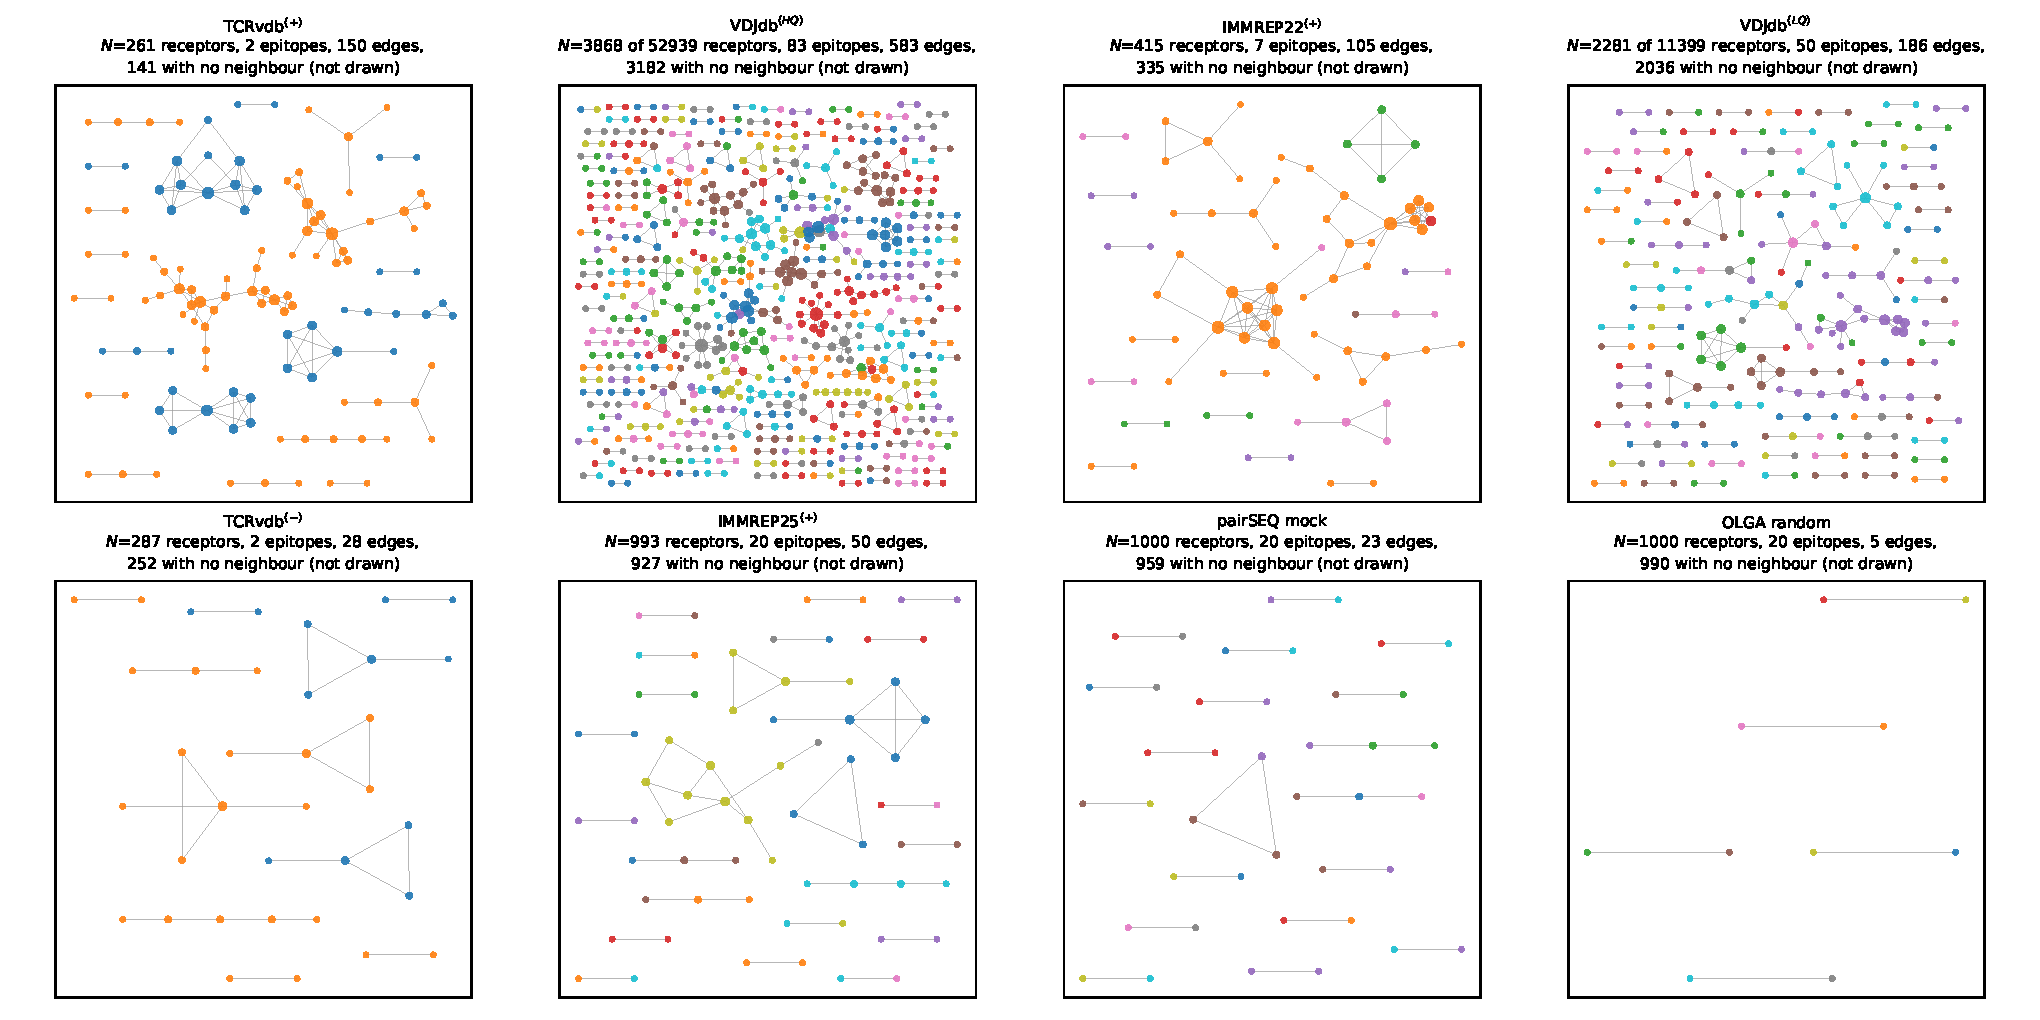
\includegraphics[width=\linewidth]{../results/figures/fig_homology_graph_TRB.pdf}
\caption{TR$\beta$ homology graph per cohort (equal sampling). Edge counts:
VDJdb-HQ $\sim$550, TCRvdb-true 75, versus immrep25 $\sim$17 and OLGA $\sim$1.}
\label{fig:homgraph}
\end{figure}
